\chapter{Introduction}

People re-identification has been an intense research topic in recent years, whose main goal is to match a given person with those persons with known labels. Person re-ID has great potential in video surveillance, target detection and tracking area. However, it is quite challenging since the accuracy is much influenced by many factors like occlusion, illumination variation, camera settings and color response. In re-ID, those images with known labels are called gallery images and the image used to know its label is called probe image. The probe image and gallery images can be from the same or different camera views, so the viewpoint and illumination between probe and gallery image can be quite different. Also for the different color response of different cameras, the shots of the same person may look different in different cameras. Besides, occlusions between camera and target person can also bring about quite much difficulty.  In a word, images of the same person may look different while images of different persons may kook quite the same. 


\begin{figure}
\centering
\begin{raggedleft}
\includegraphics[scale = 0.5]{/Users/JohnsonJohnson/Downloads/thesis_1/Figures/REIDworkflow.pdf}
%\includegraphics[width=1\linewidth]{REIDworkflow.pdf}
\vspace{1em}
\caption{A typical single shot Re-ID work flow}
\end{raggedleft}

\end{figure}

Classical people re-identification framework contains two steps, extracting the individual descriptor and comparing the similarity of different descriptors. Usually in person re-identification problem, the frames of person tracked from videos are cropped by a automatic detector or manually, so re-ID will only focus on dealing with well cropped images. 
The first task in re-ID is to design a robust descriptor to represent images. The descriptor is supposed to contain the key information for each captured person. Basically, the descriptors are supposed to be robust and discriminative. One straightforward way is to extract the color, textural information of images, then the descriptors are used to compute the similarity score. But this method turns out to be not robust caused by illumination variation  and camera color response difference and camera angle settings.  Therefore, many other advanced descriptors takes into account the correlation of color, texture and position together to improve performance.


The second one is to design the similarity computing methodology. That is, the way to compare how similar two descriptors are. Previous methods use Euclidean distance, Bhattacharyya distance and Mahalanobis distance. The Euclidean distance are mostly used to match descriptors like color and texture descriptors. However, though it's straightforward and easy, it's hard to used Euclidean distance to discriminate images. 
Many creative metric learning methods have been proposed to compute descriptor similarity. Among them the Mahanalobis distance based metric is very popular. In this method a semi-positive defined matrix $\bm{M}$ is learned while meeting certain limitations. Besides, linear discriminant analysis[] learns a subspace to minimize the within class scatter matrix while maximized inter class scatter matrix. In [] the null space is proposed that make descriptors of same class collapse into a single point while descriptors of different classes are projected to different points. 
	
\section{Basic concepts}
People re-identification can be divided into a few categories according to different conditions. Some general concepts are list below.\\
\textbf{Open set and close set re-ID} According gallery size and if the gallery size evolves, re-ID can be divided in to open set re-ID and close set re-ID. In close set re-ID, no new identities will be added to gallery set and gallery size remains the same as time goes by. Besides, the probe set will be a subset of gallery set, that means, the number of unique identities in gallery set will be equal or greater than probe set. In open set re-ID, the gallery set will evolve as time goes by. Each time a probe image is inputed to the recognition system, the system will judge if it has a corresponding match in the gallery set. If the probe image doesn't match any of the gallery images, it will be regarded as a new identity and will be added to the gallery set. Besides, the probe set is not necessarily the subset of gallery set. 

\textbf{Long term and short term re-ID} According to the time interval between gallery and probe images, re-ID can be divided into long term and short term re-ID.  In short term means the time interval between gallery and probe images are small, say a few minutes or several hours. In contrary, the long term re-ID refers to the case that the time interval between gallery and probe images are a few days or even longer. The difference brought by long time interval between gallery and probe images is the variation of individuals' clothes and appearance. If the gallery images are shot a few days ago, the same individual may have changes his suits or take off his bag, then the appearance may change a lot. In this case, it will be much more difficult to recognize the same identity in long term re-ID. Generally, in most cases we use the short term re-ID, which guarantees the appearance of same person will remain the same and we only need to consider the difference brought by other factors like viewpoint variation and occlusions.


\textbf{Single shot and multi shot re-ID} According to the size of sample set for each person, re-ID can be divided into single shot and multi shots approaches. In single shot case, only one image is provided for a person in a camera view. Single shot re-ID is challenging because only limited information can be extracted. One example is the VIPeR dataset figure[ ], in this dataset, for each person only one image is provides in each camera view. In multi shots re-ID a sequence of images are provided for a person in a camera view. Compared with single shot case, more extra information, like temporal-spatial can be extracted from the sample set. One case of multi-shot dataset is the prid\-2011 dataset which provides a long sequence for each person in a single camera view.

%-------------------------------------------------
\begin{figure}[H]

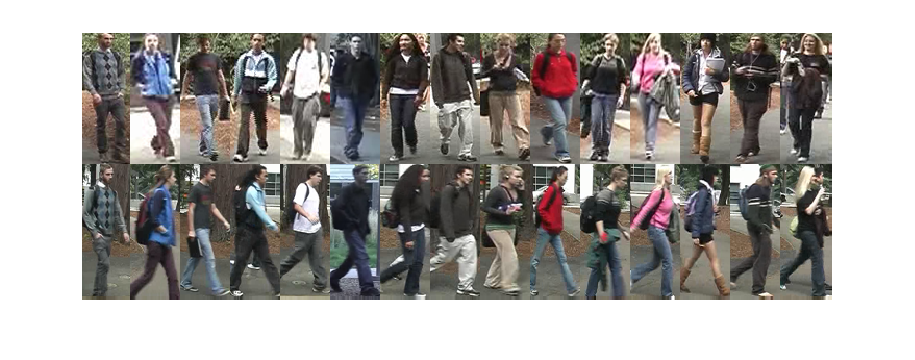
\includegraphics[width=1\linewidth]{/Users/JohnsonJohnson/Downloads/thesis_1/Figures/singleREID.eps}
\vspace{-2em}
\caption{The VIPeR dataset}

\end{figure}
%-------------------------------------------------

\begin{figure}[H]

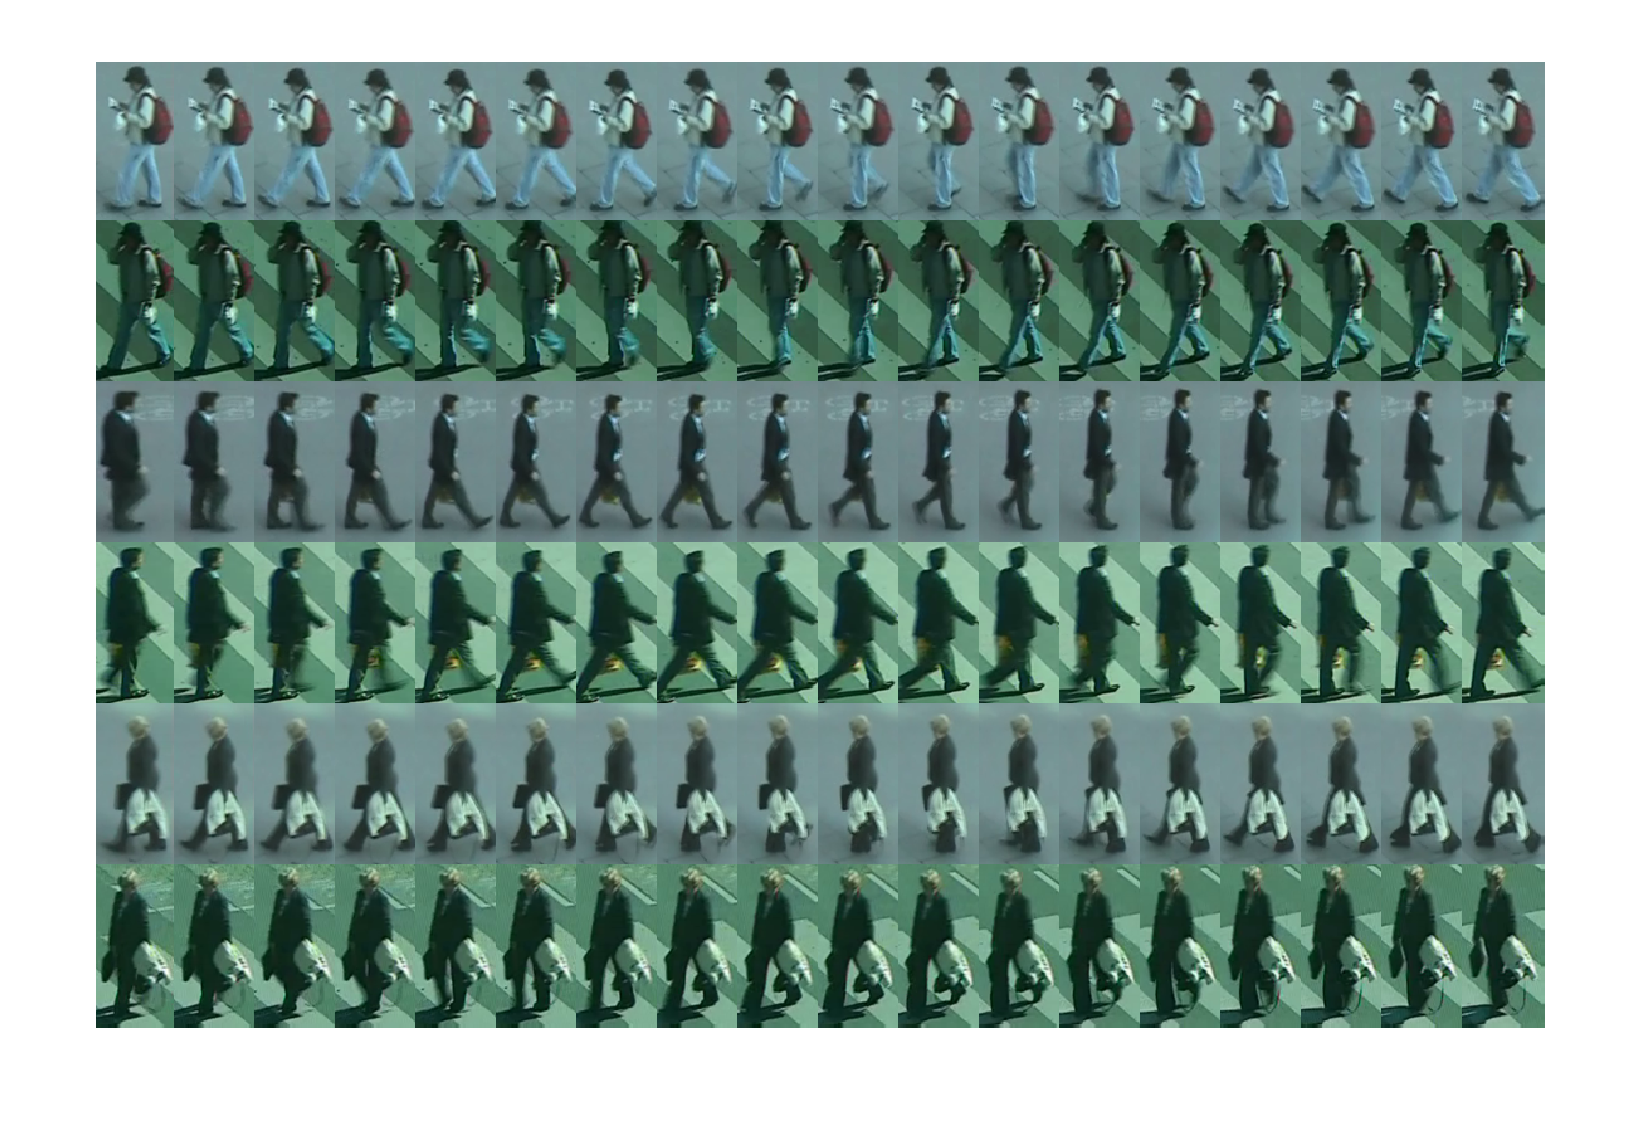
\includegraphics[width=1\linewidth]{/Users/JohnsonJohnson/Downloads/thesis_1/Figures/Multishots.eps}
\vspace{-2em}
\caption{Samples from prid\_2011 dataset}

\end{figure}


.

\section{Challenges}


\section{Proposed work}
In many previous work, the kernel local fisher discriminant analysis is used as a subspace learning method, and Euclidean distance is usually used in the subspace to measure similarity. In this thesis, the KLFDA method is used a dimension reducing method to project high dimensional descriptors to a lower dimension space. Compared with other dimension reduction methods, KLFDA is a supervised method and it take consideration of those intra and inter class information, therefore, much less information are lost after dimension reduction. Then a Mahanalobis distance based matrix $M$ is learned based on the limitation that the distance of people from same class should be at least 1 unit smaller than the distance of people from different classes. A target function that penalizes the intra-class distance and inter-class distance is created, by iterative computation, when the target function converges the matrix $M$ is thought to meet the requirement. It turns out that this metric learning have advance performance when compared with other metric learning methods.



\section{Performance measuring}

There are a few measures of re-ID, such as cumulative matching curve(CMC) curve and Receiver Operating Characteristic curve(ROC) curve. Specifically, CMC is used as a 1:m reidentification system and ROC is used for 1:1 reidentification system.  In this thesis, the cumulative matching curve is used to measure re-ID performance. The $CMC(k)$  stands for the probabilty that the right match is within the top k matches. Suppose a set of gallery $G = \{G_1,G_2,\cdots,G_m\}$ and a set of probe $P = \{P_1,P_2,\cdots,P_n\}$, for each identity $P_i$ there should be a right match in the gallery set. However, there could be identities that appear in gallery set but not in probe set. A $m\times n$ similarity matrix can be computed. Then for each probe identity $P_i$, a sorted list of gallery identities can be list as $S(P_i) = \{{G_{1},G_{2},\cdots,G_{m}}\}$ so that their similarity with $P_i$ descends. Suppose the right match of $P_i$ is at the position $k$ of $S(P_i)$, $k\le m$, then $G_i$ has a rank value of $k$. Therefore, the CMC can be calculated as 
\begin{equation}
CMC(k) = \frac{1}{n}(\#k_l\le k)
\end{equation}
where $k_l$ is the list of rank values of $P = \{P_1,P_2,\cdots,P_n\}$, and $\#k_l\le k$ means the number of rank values that is smaller than k.  Therefore, CMC curve always ascends and stops at 1.  A perfect CMC curve is supposed to have a hight rank 1 score and approaches 1 as fast as possible.




\section{Contribution}

In this paper we have two contributions, the first is we combined the KLFDA with distance comparison learning. Instead of learning the subspace with KLFDA and computing Euclidean distance in lower dimensional space, a Mahanalobis distance based matrix is learned under the limitation that the within class distance is at least 1 unit smaller than inter class distance. Compared with those advanced metrics including cross view quadratic analysis(XQDA) and Null space learning(NFST), this proposed metric learning proves to have excellent performance on VIPeR, CUHK1, prid\_2011, prid\_450s and GRID dataset.

Another contribution of this thesis is the influence of background subtraction on different descriptors are probed. We found that the background subtraction can improve the performance of some descriptors but can decrease the performance of some descriptors. The reason for this is caused by background segmentation. If descriptors are color based and don't handle texture information, like HSV histogram descriptor, background segmentation can greatly improve the performance. This comparison is shown in figure []. However, if the descriptor extracts texture information, background segmentation will decrease its performance since the imperfect segmentation will cause many small black dots in foreground area, which will cause gigantic textural information variation. 


Because segmentation algorithm will bring about more 

\section{Thesis organization}
In this thesis, Chapter 2 will give a brief introduction of previous work. Chapter 3 will explain the implementation of the hierarchical gaussian descriptors used in this thesis. In Chapter 4 a detailed introduction of the kernel local fisher local discriminant analysis will be presented, and a detailed explanation will also be presented about the metric learning on the lower dimension space based on relative distance comparison.
In Chapter 5 the used datasets and parameters and other experiment settings will be explained, and a detailed analysis of results is presented here. At last, the conclusion is given in Chapter 6.




